\documentclass[a4paper,11pt,twoside]{article}
\usepackage[utf8]{inputenc}	% Text coding
\usepackage[T1]{fontenc}
\usepackage{lmodern}
\usepackage[czech]{babel}
\usepackage{epsfig}
\usepackage{amsfonts,amsmath,amssymb}
\usepackage{graphicx}
\usepackage[unicode]{hyperref}
\usepackage{indentfirst}
\usepackage{fancyhdr}
\usepackage{xifthen}
\usepackage{amsthm,thmtools}
\usepackage{bold-extra}
\usepackage[dvipsnames]{xcolor}
\usepackage[subrefformat=simple,labelformat=simple]{subcaption} % Instead of subfigure
\usepackage{listings}
\usepackage{comment}
\usepackage{titlesec}
%\usepackage{showlabels}

\hypersetup{
	pdftitle={Využití počítačů ve fyzice},
	pdfauthor={Pavel Stránský},
	pdffitwindow=true,
	colorlinks=true,
	urlcolor=cyan,
	linkcolor=red,
	citecolor=green,
	filecolor=magenta
}

\graphicspath{{figures/}}

\lstdefinestyle{listingsstyle}{
    basicstyle=\ttfamily,
    breakatwhitespace=false,         
    breaklines=true,                 
    keepspaces=true,                 
    showspaces=false,                
    showstringspaces=false,
    showtabs=false,                  
    tabsize=2,
    columns=fullflexible
}

\lstset{style=listingsstyle}

%\babelhyphenation[czech]{ma-te-ma-tic-kých}

\renewcommand\thesubfigure{(\alph{subfigure})}

% Page size
\addtolength{\topmargin}{-1.5cm} %\addtolength{\textheight}{-10cm}
\addtolength{\textwidth}{4cm} \addtolength{\textheight}{4cm} % Width and height of the text
\addtolength{\voffset}{-0.5cm} % Top margin
\addtolength{\hoffset}{-2cm}
\setlength{\headheight}{15pt}

\pagestyle{fancy}

\DeclareMathOperator{\e}{e}

\def\vector#1{\boldsymbol{#1}}								% Vector
\renewcommand{\d}{\mathrm{d}}
\newcommand{\derivative}[3][]{\ifthenelse{\isempty{#1}}	    % Normal derivative
	{\frac{\d{#2}}{\d{#3}}}
	{\frac{\d^{#1}{#2}}{\d{#3}^{#1}}}
}
\newcommand{\im}{\mathrm{i}}

\def\makematrix#1{\begin{pmatrix}#1\end{pmatrix}}       % Matrix
\def\abs#1{\left|#1\right|}
\def\probability#1{\mathrm{Pr}\left[#1\right]}
\def\expectation#1{\mathrm{E}\left[#1\right]}
\def\dispersion#1{\sigma_{#1}^{2}}

\def\code#1{\textnormal{\texttt{#1}}}
\def\file#1{\textnormal{\textbf{\texttt{#1}}}}

\def\abbreviation#1{\textnormal{\textsc{#1}}}

\long\def\python#1{{\color{ForestGreen}#1}}

\newtheoremstyle{spaced}
{5pt}{5pt}{\itshape}{}{\bfseries}{:}{.5em}{}

\newtheoremstyle{red}
{5pt}{5pt}{\itshape}{}{\bfseries}{:}{.5em}{}

\newtheoremstyle{blue}
{5pt}{5pt}{\itshape\color{blue}}{}{\bfseries\color{blue}}{:}{.5em}{}

\begin{document}

\theoremstyle{spaced}
\newtheorem{example}{Příklad}[section]

\theoremstyle{red}
\newtheorem{task}{Úkol}[section]

\theoremstyle{blue}
\newtheorem{solution}{Řešení}[section]

\title{Zápisky k předmětu Využití počítačů ve fyzice}
\date{\today}
\author{Pavel Stránský}

\maketitle
\tableofcontents

\newcommand{\sectionbreak}{\clearpage}

\section{Instalace používaných nástrojů}
\label{sec:Instalace}
    Příklady k cvičení budou demonstrovány v nejnovější verzi programovacího jazyka \href{https://python.org}{Python}.
    Jako vývojové prostředí doporučuji \href{https://code.visualstudio.com}{Visual Studio Code}.
    Tento volně dostupný program lze nainstalovat na všechny neužívanější operační systémy (Linux, Windows, macOS).    
    Má nepřeberné možnosti při editaci zdrojových souborů, překladu a ladění snad ve všech známých programovacích jazycích.
    Bohaté možnosti nastavení umožnují přizpůsobit si práci svým potřebám (například zvýrazňování syntaxe, klávesové zkratky či vzhled prostředí).
    Pomocí doplňků ho můžete integrovat s dalšími službami, například s verzovacím programem Git, či vzdálenými repozitáři, čehož také využijeme.
    Komunita, která toto vývojové prostředí používá a spravuje, je obrovská, což zaručuje dobrou podporu a rychlé přidávání nových funkcí.

\subsection{Instalace Pythonu}
\label{sec:InstalacePython}
    Instalační soubor pro svůj operační systém stáhnete ze stránky \href{https://python.org}{python.org}.
    Při instalaci na počítač s Windows doporučuji zvolit \uv{Add Python to PATH}, což zjednoduší práci s Pythonem z příkazové řádky, a na poslední obrazovce zvolit \uv{Disable path length limit}:
    \begin{center}
        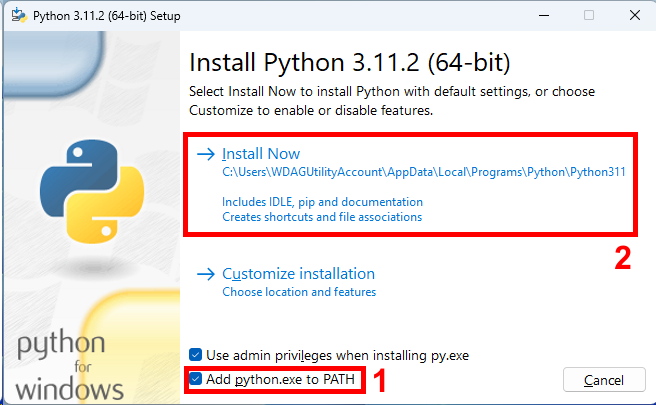
\includegraphics[width=0.495\linewidth]{PythonInstallPath.png}
        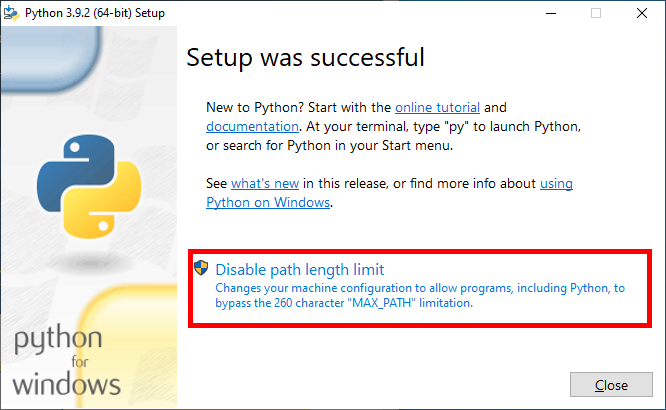
\includegraphics[width=0.495\linewidth]{PythonInstallPathLimit.png}
    \end{center}
    Pro ověření instalace napíšeme v příkazové řádce příkaz \code{python}.\footnote{Na počítačích s Linuxem je příkaz v terminálu \code{python3}.}
    Tím se spustí \abbreviation{REPL}\footnote{{\bf R}ead-{\bf E}valuate-{\bf P}rint-{\bf L}oop.} Pythonu, ve které můžeme již psát všechny příkazy programovacího jazyka, které se po zadání ihned provedou a vypíšou výsledek.

\subsubsection{Instalace doplňujících knihoven}
\label{sec:pip}
    Samotná instalace Pythonu obsahuje jen minimální množství nejnutnějších knihoven.
    My budeme využívat ještě následující rozšiřující knihovny:
    \begin{itemize}
        \item \file{\href{https://numpy.org}{NumPy}} ({\bf Num}erical {\bf Py}thon: numerická matematika, řady a vícedimenzionální datové typy),
        \item \file{\href{https://scipy.org}{SciPy}} ({\bf Sci}entific {\bf Py}thon: algoritmy pro optimalizaci, statistiku, řešení diferenciálních rovnic, lineární algebru, atd.),
        \item \file{\href{https://matplotlib.org}{Matplotlib}} (vizualizace, grafy).
    \end{itemize}
    K jejich doinstalování slouží modul \code{pip}.
    V příkazové řádce napíšeme
    \begin{lstlisting}
        python -m pip install numpy scipy matplotlib
    \end{lstlisting}
    čímž se nainstalují naráz všechny tři knihovny.\footnote{
        Pokud na počítači s Linuxem uvedený postup nebude fungovat, je potřeba nejprve nainstalovat instalátor \file{pip} pomocí příkazu \code{sudo apt install python3-pip}.
        Pak lze použít buď výše uvedený příkaz, nebo stručnější \code{pip3 install numpy}.
    }
    
    Existuje samozřejmě celá řada dalších užitečných a používaných knihoven, jako je například \file{\href{https://pandas.pydata.org/}{Pandas}} pro analýzu dat nebo \file{\href{https://www.sympy.org/}{SymPy}} pro symbolické výpočty, na které v tomto kurzu nedojde.

\subsection{Instalace Visual Studio Code}
    Instalace jazyka Python obsahuje jednoduché vývojové prostředí nazvané \abbreviation{\href{https://docs.python.org/3/library/idle.html}{IDLE}}.\footnote{
        {\bf I}ntegrated {\bf D}evelopment and {\bf L}earning {\bf E}nvironment.
    }
    To však poskytuje jen omezené možnosti co se týče ladění, psaní rozsáhlejších projektů s více zdrojovými soubory nebo integrace s verzovacími programy.

    Pro serióznější práci budeme používat \href{https://code.visualstudio.com}{Visual Studio Code} s doplňkem pro programovací jazyk Python.
    Instalační soubor stáhnete ze stránky \href{https://code.visualstudio.com}{code.visualstudio.com}.
    Během instalace na počítač s Windows doporučuji zvolit obě možnosti \uv{Add Open with Code action to...},
    \begin{center}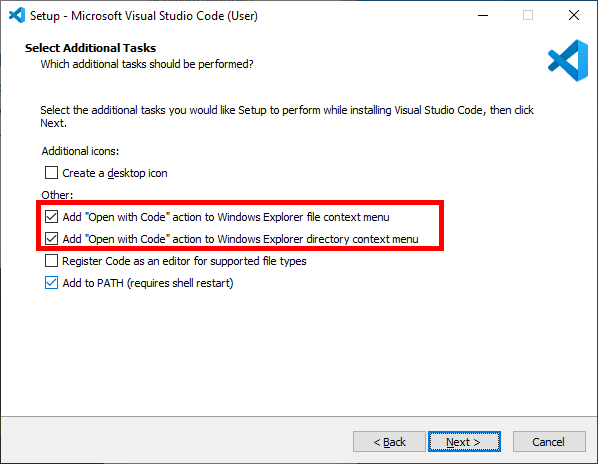
\includegraphics[width=0.5\linewidth]{VSCodeInstall.png}\end{center}
    což zjednoduší otevírání složek s projekty nebo samostatných souborů pomocí pravého tlačítka myši.

    Na operačním systému Linux je nejjednodušší provést instalci pomocí Snap Store příkazem v terminálu
    \begin{lstlisting}
        sudo snap install --classic code
    \end{lstlisting}
    nebo použít tento \href{https://code.visualstudio.com/docs/setup/linux}{návod}.

\subsubsection{Instalace doplňku pro Python}
    \begin{center}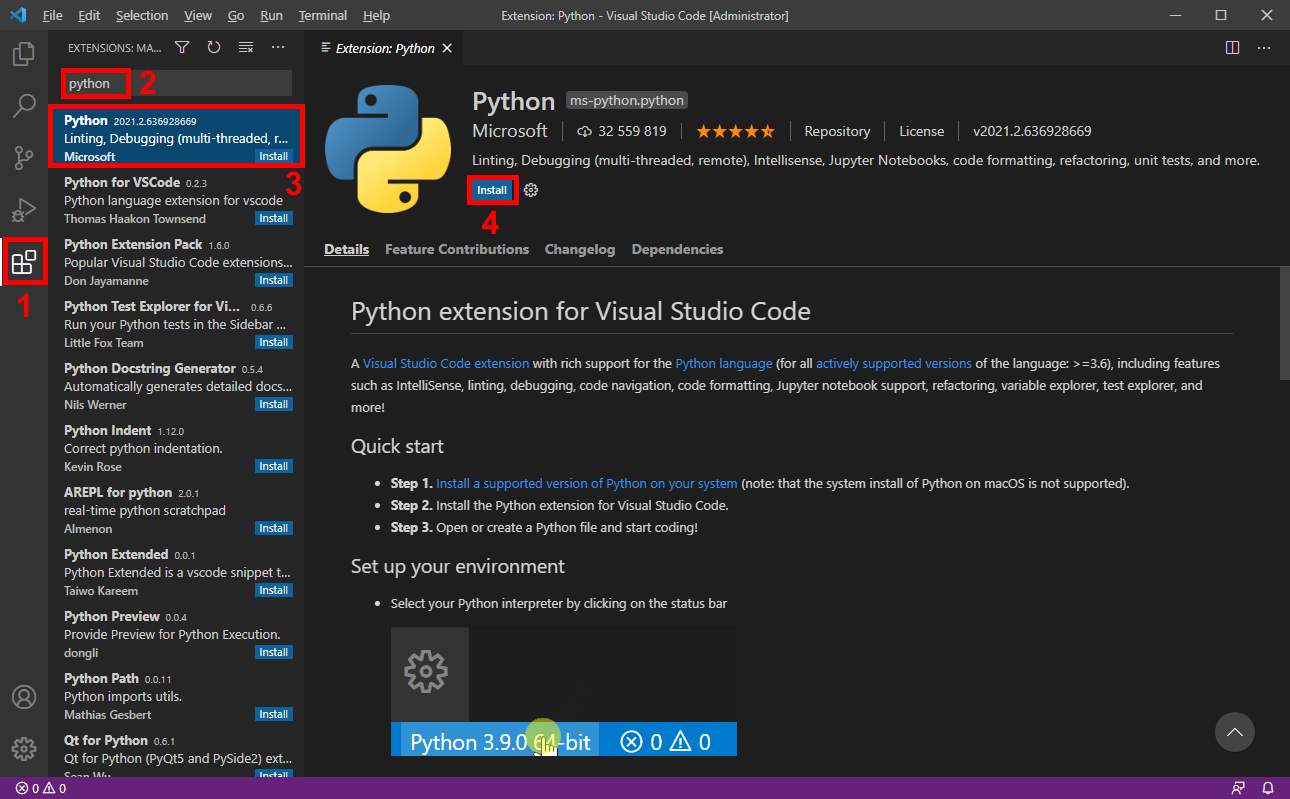
\includegraphics[width=\linewidth]{VSCodeInstallPython.png}\end{center}
    Ke správě doplňků (extensions) se dostanete kliknutím na ikonku {\color{red} 1} nebo stisknutím \code{Ctrl+Shift+X}. 
    Vyhledáte doplněk \href{https://marketplace.visualstudio.com/items?itemName=ms-python.python}{Python} {\color{red} 2} od Microsoftu, vyberete ho {\color{red} 3} a nainstalujete {\color{red} 4}.

\subsection{Instalace Git}
    Instalační soubor verzovacího systému \href{https://git-scm.com}{Git} stáhnete z webové stránky \href{https://git-scm.com}{git-scm.com}.
    K instalaci Gitu potřebujete administrátorská práva.
    
    V následujícím postupu zobrazuji jen ty snímky obrazovky, na kterých je vhodné vybrat jinou volbu, než jaká je instalátorem standardně nabízena.
    \begin{center}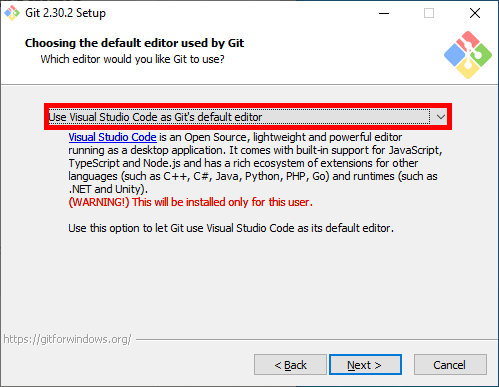
\includegraphics[width=0.5\linewidth]{GitInstallEditor.png}\end{center}
    Jako editor zvolíme dříve nainstalované Visual Studio Code.
    Systém Git vyžaduje editor jednak pro povinný komentář každé zapsané změny (commit), jednak pro ošetření kolizí při slučování větví (merge).
    \begin{center}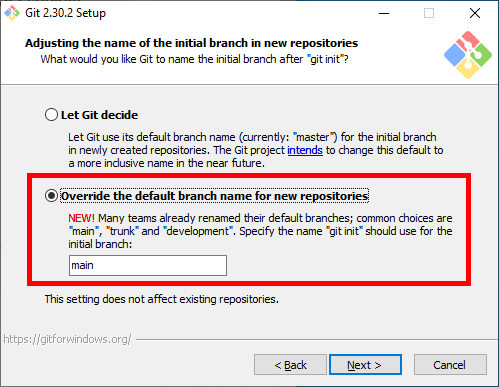
\includegraphics[width=0.5\linewidth]{GitInstallMain.png}\end{center}
    Hlavní větev repozitáře se donedávna standardně jmenovala \code{master}.
    Vzhledem k negativním konotacím tohoto slova v angličtině se přechází na neutrálnější označení.
    Nejběžnější je \code{main}, na které již přešel i populární správce vzdálených repozitářů \href{https://github.com}{GitHub}.
    Doporučuji tedy zvolit pojmenování \code{main}.

    Všechna nastavení lze samozřejmě kdykoliv po instalaci změnit.

\section{Úvod do používaných nástrojů}
    V této sekci naleznete základy použití verzovacího systému Git a úvod do syntaxe a idiomatiky jazyka Python.
    Na rozdíl od zbytku poznámek bude tato sekce v průběhu cvičení postupně doplňována podle toho, s jakými technikami se seznámíme v hlavní části cvičení.

\subsection{Verzovací systém Git}
    Každý si patrně už někdy v životě zasteskl, že nemá uložené dřívější verze svých souborů.
    Změny, které se ukazují být nevhodné či provedené omylem (kočka nepozorovaně přejde po klávesnici a my pak soubor uložíme), kamarád, který z nějakých důvodů chce tu verzi vašeho programu, kterou jste mu poskytli před rokem, a vy jste mezitím kód zásadně přepsali, to vše jsou důvody k předsevzetí nějakým způsobem důležité milníky v práci na projektu archivovat.

    Triviální verzování může spočívat například v ručním ukládání kopií projektu s daty či jinými označeními jednotlivých verzí.
    Takovýto postup je ale velmi těžkopádný, jelikož v každé kopii musí být uloženy všechny soubory projektu, i pokud se v nich od předchozí verze nic nezměnilo.
    Obtížně se vyhledává, co přesně se mezi jednotlivými verzemi změnilo a kdo změnu provedl, pokud na projektu pracuje větší tým, přičemž obtížnost roste s velikostí a komplexností projektu.
    Pro usnadnění uchovávání historie změn proto vznikly verzovací systémy.    

    Verzovací systém pomáhá udržet historii změn souborů projektu, přičemž ke každému snímku historie se lze vrátit.
    Vše provádí chytře a v maximální míře automaticky.
    Systém sám sleduje, v jakých souborech byly provedeny změny.
    Pokud se jedná o textový soubor, umí porovnat aktuální a libovolnou historickou verzi řádek po řádku a zvýraznit odlišnosti.
    Umožňuje pracovat s nezávislými vývojovými větvemi (\emph{branches}), ve kterých lze například zkoušet různý přístup k řešení daného problému a mezi kterými lze jednoduše přepínat.
    Vybrané řešení lze pak snadno začlenit (\emph{merge}) do hlavní vývojové větve.

    Soubory projektu a informace o jejich historických změnách se nazývá souhrnně \emph{repozitář}.
    V něm se uchovávají nejen verze souborů, ale také údaje o tom, kdo a kdy změny provedl.
    To předurčuje verzovací systémy pro efektivní správu týmových projektů, kdy každý člen týmu pracuje na určité části projektu a své změny následně do projektu včleňuje.

    My budeme používat verzovací systém \href{https://git-scm.com}{Git}.
    Ten patří mezi \emph{distribuované} verzovací systémy, což znamená, že každý uživatel má na svém počítači celý obsah repozitáře a pouze ve chvílích, kdy uzná za vhodné nebo kdy je k tomu příležitost, může své změny synchronizovat se \emph{vzdáleným repozitářem}, ve kterém se shromažďují změny od všech členů týmu, začleňují do hlavní vývojové větve projektu a hlídají případné kolize.
    Výhody tohoto přístupu oproti centrálně řízeným verzovacím systémům jsou následující:
    \begin{enumerate}
        \item Práce na projektu nevyžaduje připojení k nějakému centrálnímu serveru s repozitářem, a tedy můžete pracovat offline klidně někdě v džungli nebo na Marsu.
        \item Není potřeba spravovat zvlášť server s repozitářem a zvlášť klientské počítače. Vše je na jednom místě.
        \item Při práci na týmovém projektu není případná porucha počítače spojená se ztrátou dat žádná katastrofa, protože ostatní kolegové mají celou kopii repozitáře na svých počítačích.
    \end{enumerate}
    Git nejefektivněji funguje na textové soubory, ale zvládne verzovat i soubory binární (například obrázky).

    Git je v dnešní době jeden z nejpopulárnějších verzovacích systémů.
    Pod jedho správou jsou vyvíjeny i velké projekty, například samo \href{https://github.com/microsoft/vscode}{Visual Studio Code}.
    Tento projekt je navíc otevřený (open source), což znamená, že kdokoliv, tedy i vy nebo já, má přístup k celému repozitáři, tedy ke všem zdrojovým kódům a k jejich kompletní historii. 
    Může se do práce na projektu zapojit, přispět k jeho vývoji a začít psát historii sám.
    
    Program Git pochází z prostředí Linuxu, a proto je navržený tak, aby se s ním dalo pracovat z příkazové řádky (terminálu) pomocí jednoduchých textových příkazů.
    Tímto způsobem lze používat všechny dostupné funkce Gitu.
    My se s nejdůležitějšími funkcemi seznámíme právě pomocí textových příkazů, protože na nich se nejlépe naučí, jak tento Git funguje a jaké jsou jeho možnosti.
    Jakmile si člověk ujasní principy verzování pomocí Gitu, nabízí se spousta nástrojů a doplňků pro různé programy, které práci s repozitáři usnadní a zrychlí.
    Obsluha Git repozitářů je ostatně integrována i do vývojového prostředí Visual Studio Code.

    Na stránkách projektu Git najdete \href{https://git-scm.com/book/en/v2}{podrobný interaktivní návod} ke všem funkcím verzovacího systému (a to částečně i v \href{https://git-scm.com/book/cs/v2}{češtině}).

\subsubsection{Prvotní nastavení}
    Git nelze používat do té doby, než jsou nastaveny základní informace o uživateli.
    To se provede pomocí příkazů v příkazové řádce (terminálu)
    \begin{lstlisting}
        git config --global user.name "..."
        git config --global user.email "..."
    \end{lstlisting}
    přičemž za ... doplníte své jméno (přezdívku) a email.
    Těmito údaji se podepisují všechny zapsané změny v repozitáři.
    Pokud tedy spolupracujete na projektu s jinými lidmi, je dobré zvolit takové údaje, pomocí kterých vás kolegové snadno identifikují a úspěšně kontaktují.

    Výpis všech nastavení získáte příkazem
    \begin{lstlisting}
        git config --global
    \end{lstlisting}
    Uvidíte, že v mezi nastaveními je i název hlavní větve repozitáře (\code{init.defaultbranch=main}) a cesta k nastavenému textovému editoru (v našem případě Visual Studio Code).

    Všechna nastavení a práci s příkazem \code{config} najdete v tomto \href{https://git-scm.com/docs/git-config}{podrobném návodu} nebo zadáním příkazu
    \begin{lstlisting}
        git help config
    \end{lstlisting}

\subsubsection{.gitignore}
    Překladače programovacích jazyků často vytvářejí v adresáři vašeho projektu dočasné pomocné soubory, které nechcete, aby se staly součástí repozitáře (tyto soubory nenesou žádnou relevantní informaci, navíc mohou na různých počítačích vypadat jinak podle toho, jaký překladač či jaké vývojové prostředí zrovna použijete).
    Abyste mohli používat příkazy pro hromadné sledování či zapisování souborů \code{git add *} či \code{git commit -a}, musíte GITu naznačit, jaké soubory má ignorovat.
    K tomu slouží soubor \code{.gitignore}.
    
    Každé pravidlo v souboru \code{.gitignore} zabírá jeden řádek.
    Řádek, který začíná znakem \#, je ignorován a může sloužit například jako komentář.
    Příklady jednotlivých řádků:
    \begin{itemize}
    \item \code{tajne.txt}
        
        Ignoruje soubor s názvem \code{tajne.txt} (může obsahovat třeba přihlašovací údaje k nějaké službě a ty rozhodně nechceme sdílet ani archivovat; nezapomeňte, že co je jednou zapsané v repozitáři, z něj až na výjimky nelze odstranit).

    \item \code{*.log}
    
        Ignoruje všechny soubory s příponou \code{log},

    \item \code{!important.log}

        ale neignoruje soubor \code{important.log}.

    \item \code{*.[oa]}

        Ignoruje všechny soubory s příponou \code{o} nebo \code{a}.

    \item \code{temp/}

        Ignoruje všechny soubory v podadresáři \code{temp}.

    \item \code{doc/**/*.pdf}
    
        Ignoruje všechny soubory s příponou \code{pdf} v podadresáři \code{doc} a ve všech jeho podadresářích.
        Neignoruje však soubory s příponou \code{pdf} v hlavním adresáři projektu.
    \end{itemize}
    Další příklady jsou například~\href{https://www.atlassian.com/git/tutorials/saving-changes/gitignore}{zde}.

    Pokud na GitHubu zakládáte nový projekt, můžete upřesnit, jaký programovací jazyk budete používat a GitHub automaticky vytvoří optimální soubor \code{.gitignore}.

    {\color{ForestGreen}
    \begin{task}
        Podívejte se do souboru \code{.gitignore} v repozitáři k těmto zápiskům.
        Zatímco Python si téměř žádné pomocné soubory nevytváří, {\LaTeX} jich generuje požehnaně.
        Proto je tento soubor celkem dlouhý. 
    \end{task}
    }

\subsubsection{Cheat Sheet}
    Pro snadnou orientaci v použití Gitu bez nutnosti pamatovat si všechny příkazy je dostupný \href{https://training.github.com/downloads/github-git-cheat-sheet.pdf}{Git Cheat Sheet} nebo \href{https://ndpsoftware.com/git-cheatsheet.html}{tento interaktivní web}.

\subsection{Programovací jazyk Python}
    Python je v dnešní době velmi populární programovací jazyk, který pronikl do spousty rozmanitých odvětví, a to zejména díky bohatosti a pokročilosti knihoven, které jsou vyvíjeny komunitou a jsou díky tomu aktuální a odladěné (či průběžně odlaďované).
    Python existuje na mnoha platformách od osobních počítačů po mikrokontroléry a dá se v něm naprogramovat téměř cokoliv: pokročilé vědecké výpočty používající nejnovější numerické algoritmy, dobře vypadající grafy, statistická analýza, analýza velkých dat a strojové učení, ale také webové služby, okénkové programy či editace obrázků a videí.
    Je běžné, že i komerční programy obsahují Python coby skriptovací jazyk, čímž umožňují uživateli používat své vlastní kódy \uv{uvnitř} komerčního produktu a integrovat různé programy mezi sebou.\footnote{
        Jako příklad poslouží nejnovější verze programu \href{https://www.wolfram.com/language/12/external-system-integration/evaluate-python-in-a-notebook.html}{Mathematica}, \href{https://www.originlab.com/doc/python/Run-Python-in-Origin}{Origin} či \href{https://developer.sas.com/guides/python.html}{SAS}.
    }
    
    Python lze charakterizovat jako jazyk:
    \begin{itemize}
        \item 
            \emph{Interpetovaný}, což znamená, že provádění programů probíhá přímo ze zdrojového kódu.\footnote{
                Mezi další známé interpetované jazyky patří napříkad JavaScript nebo PHP.
            }
            Ke spouštění kódů je tedy potřeba mít nainstalovaný interpret, což jsme učinili v sekci~\ref{sec:InstalacePython}.
            Pokud kód obsahuje syntaktickou chybu, je odhalena až ve chvíli, kdy se na ni interpret při provádění kódu narazí.
            U interpretovaných jazyků se neztrácí čas překladem do strojového kódu a je pro ně přirozené dynamické typování proměnných.
            Tím, že interpet čte text kódu příkaz po příkazu, je provádění programů pomalejší, ale vzhledem k tomu, že velká část časově náročných funkcí a knihoven bývá napsána v rychlejších programovacích jazycích, není to zásadní nevýhoda.
            
            Opakem intepretovaných jazyků jsou jazyky kompilované, přičemž kompilace se provádí buď přímo do strojového kódu daného procesoru\footnote{Například C/C++, Pascal nebo Fortran.} nebo do mezikódu. Ten  ke spuštění vyžaduje dodatečnou kompilaci, která však může být vysoce optimalizovaná přímo pro danou hardwarovou konfiguraci použitého počítače.\footnote{Zde se jedná napřílad o jazyky Java, C\# a celý .NET framework nebo Julia.}

        \item 
            \emph{Dynamicky typovaný}, což znamená, že proměnná nemusí mít předem daný typ a typ proměnné se může za běhu programu dokonce měnit.
        
        \item 
            \emph{S automatickou správou paměti}, takže programátor se nemusí starat o alokování a uvolňování paměti. 
            Python při inicializaci proměnné paměť alokuje automaticky a ve chvíli, kdy proměnnou přestaneme používat, paměť uvolní.\footnote{Algoritmus se nazývá \emph{Garbage collection}.} 

        \item
            V Pythonu lze pythonovským způsobem používat tři základní programovací paradigmata: \emph{procedurální, objektové a funkcionální}.
    \end{itemize}
         
    Python klade důraz na jednoduchost, stručnost a čitelnost kódu.
    Filosofie programovacího jazyka je shrnuta v \href{https://www.python.org/dev/peps/pep-0020/}{Zenu Pythonu},\footnote{Zen se také vypíše, pokud do svého kódu zadáte \code{import this}.} se kterým vám doporučuji se seznámit.

\subsubsection{Vytvoření a spuštění kódu}
    Ve Visual Studio Code vytvoříme nový soubor a uložíme si ho s příponou \code{*.py}. 
    Podle této přípony VS Code pozná, že se jedná o pythonovský kód a použije k práci s ním správný doplněk.
       
    Hotový kód lze spustit ve VS Code jedním z následujících tří způsobů.
    \begin{enumerate}
        \item 
            \emph{Kliknutím na zelenou šipku na nástrojové liště}:
            Tímto způsobem se spustí celý soubor kódu.
        \item
            \emph{Stiskem \code{F5}} (a výběrem Python File): Kód se spustí v režimu ladění (debugger).
            Zastaví se na každém kontrolním bodě (breakpoint, který se vloží na vybranou řádku kódu klávesou \code{F9}) nebo na každé chybě.
            Pro pokračování provádění kódu stačí stisknout buď znovu \code{F5}, nebo \code{F10} či \code{F11} pro jeden krok.

        \item
            \emph{Označením části kódu a stiskem Ctrl+Enter}: V okně \code{TERMINAL} spustí \abbreviation{REPL} Pythonu a v něm označenou část kódu.
            \abbreviation{REPL} se po provedení kódu nezavře, takže v něm lze psát dodatečné příkazy.
            Pro ukončení \abbreviation{REPL} do něj stačí napsat \code{exit()} nebo v něm stisknout \code{Ctrl+Z} a potvrdit.
            \abbreviation{REPL} musí být ukončen, než se použije jakákoliv z dvou dříve popsaných metod spuštění kódu.
    \end{enumerate}

\subsubsection{Základy syntaxe Pythonu}
    Soubor se vzorovými příklady najdete v repozitáři ke cvičení: \file{\href{https://github.com/PavelStransky/PCInPhysics2021/blob/main/python/PythonBasics.py}{PythonBasics.py}}.\footnote{
        Vzorový soubor je inspirován příkladem \href{https://learnxinyminutes.com/docs/cs-cz/python/}{Nauč se Python v Y minutách}.
    }
    Doporučuji vám si ho stáhnout nebo jeho obsah překopírovat a důsledně si ho řádek po řádku projít a spouštět nejlépe pomocí označení a stiskem \code{Ctrl+Enter}, jak bylo popsáno v předchozí sekci.
    Některé části kódu odkazují na proměnné zavedené v dřívější části souboru, proto kód procházejte postupně od začátku do konce.

    Z vzorového kódu bych vypíchl následující body:
    \begin{enumerate}
        \item 
            \emph{Základní datové typy a operátory}: Zaměřte se na možnosti formátování řetězců. 
            Python obsahuje jen dva základní číselné typy: \code{int} a \code{float}.
            Zbytek je podobný jako v jiných programovacích jazycích.

        \item
            \emph{Proměnné a kolekce}: 
            Důležité standardní kolekce jsou \emph{seznam} (list) [...] a \emph{slovník} (dicctionary) \{...\}.
            Dále existuje typ \emph{n-tice} (tuple) (...) a \emph{množina} (set) \{...\}.
            O jaký typ kolekce se jedná poznáte podle typu závorek, kterými je uzavřena.
            Python nabízí bohaté možnosti indexování prvků kolekcí.

            Python nemá typ \uv{řada} (jedno či vícerozměrný soubor hodnot stejných typů).
            Ten je implementován až v rozšiřujících knihovnách, například v knihovně \file{numpy}, které se budeme věnovat později.
            
        \item
            \emph{Podmínky a cykly}:
            Příkaz uvozující blok kódu vždy končí znakem \uv{:}.
            Každý blok je definován svým odsazením, které musí být na každém řádku stejné
            (tj. musí obsahovat stejný počet odsazujících znaků, mezi které patří buď mezera nebo tabulátor).
            Konvence je používat k odsazení \href{https://www.python.org/dev/peps/pep-0008/#indentation}{4 mezery}.

            Cykly jsou možné pouze přes iterovatelné objekty.
            Pro cyklus přes přirozená čísla (indexy) musíme vytvořit odpovídající iterovatelný objekt příkazem \code{range}.
            V drtivé většině se lze při programování v Pythonu indexům zcela vyhnout.

        \item 
            \emph{Funkce}: Python umožnuje velkou variabilitu co se týče argumentů funkce a návratových hodnot díky své funkci automatického sbalení a rozbalení kolekcí.
            Funkce se navíc chová jako objekt, lze ji tedy přiřadit jakékoliv proměnné.
            To je jeden z prvků funkcionálního programování.

            Funkcionální programování také obsahuje koncept anonymní funkce, což je jednoduchá funkce definovaná na jednom řádku, která nemá vlastní jméno.
            V Pythonu se vytváří pomocí klíčového slova \code{lambda}.

        \item 
            \emph{Moduly}: Při programování je důležité vhodně strukturovat kód.
            Python obsahuje jednoduchý koncept modulů, přičemž každý soubor s příponou \code{*.py} lze použít jako modul.
            Modul je vlastně speciální typ objektu.

            Dobře se seznamte se způsoby, jak modul načíst a používat, jelikož většina funkcí Pythonu se nachází právě v modulech.
            Jedná se například o matematické funkce v modulu \file{math} nebo rozšiřující knihovny \file{numpy}, \file{scipy} a \file{matplotlib}.

        \item 
            \emph{Třídy}: Python umožňuje objektově orientované programování.
            Práce s třídami se však v mnohém liší od striktně objektově orientovaných programovacích jazyků, jakými jsou například C++, C\# nebo Java.
            Důležitý rozdíl je například v přístupnosti atributů (všechny atributy v Pythonu jsou veřejné).
            Rovněž dědičnost a dědění metod se chová odlišně.
            Dále je nutné pamatovat na to, že každá metoda třídy musí mít v deklaraci jako první argument odkaz na instanci, se kterou je volána (konvenčně se označuje \code{self}).
            Ve vzorovém kódu je k objektovému programování opravdu jen to nejnutnější minimum.
            Pokud chcete v Pythonu využívat objekty seriózně, doporučuji pročíst si odpovídající \href{https://docs.python.org/3/tutorial/classes.html}{kapitolu v manuálu}.
    \end{enumerate}

    Uvedený kód s příklady obsahuje jen ty struktury jazyka Python, které budeme používat.
    V budoucích cvičeních se ještě seznámíte se \emph{správou kontextu} (klíčové slovo \code{with}).
    Python umožňuje navíc 
    \begin{itemize}
        \item ošetření chyb pomocí \emph{výjimek} (klíčová slova \code{raise}, \code{try}, \code{except}, \code{finally}),
        \item tvorbu \emph{generátorů} (klíčové slovo \code{yield}),
        \item \emph{asynchronní programování}, korutiny a úkoly (klíčová slova \code{await}, \code{async})
        \item či tvorbu a použití \emph{dekorátorů}.
    \end{itemize}
    Pro plné ovládnutí jazyka vám doporučuji se v budoucnu s těmito koncepty seznámit, a to buď ze specializovaných přednášek, z tutoriálů a návodů na webu, nebo studiem cizích kódů.

    Na oficiálních stránkách Pythonu najdete \href{https://docs.python.org/3/tutorial/}{tutoriál k nejnovější verzi programovacího jazyka}.

\subsubsection{Pojmenování proměnných a formátování}
    Formátování kódu Pythonu je celkem volné.
    Povinné je dodržet jen správné odsazení bloků.
    Pro snazší čitelnost kódu byla nicméně vytvořena řada doporučení, která najdete souhrnně na stránce \href{https://www.python.org/dev/peps/pep-0008}{PEP 8}.\footnote{\abbreviation{PEP} = {\bf P}ython {\bf E}nhancement {\bf P}roposal}
    Python obsahuje dokonce knihovnu \file{\href{https://pypi.org/project/autopep8/}{autopep8}}, která váš zdrojový soubor podle těchto pravidel naformátuje.
    Automatické formátování podle PEP 8 lze nastavit i ve \href{https://code.visualstudio.com/docs/python/editing#_formatting}{Visual Studiu Code}.
        
    Pro pojmenování proměnných existuje jediné závazné pravidlo, které zní, že indentifikátor se nesmí shodovat s žádným z \href{https://docs.python.org/3/reference/lexical_analysis.html#keywords}{35 klíčových slov} jazyka.
    Kromě toho jsou ve výše uvedeném dokumentu další nezávazná pravidla k pojmenování proměnných:\footnote{
        Čitelnosti různých stylů pojmenování proměnných se věnují i seriózní vědecké články, například
        \url{http://www.cs.kent.edu/~jmaletic/papers/ICPC2010-CamelCaseUnderScoreClouds.pdf}.
    }
    \begin{itemize}
        \item
            \emph{Proměnné a funkce} se doporučuje pojmenovávat malými písmeny a jednotlivá slova spojovat podtržítky, tzv. underscore style (například \code{pocet\_bodu}).
        \item
            \emph{Konstanty} se doporučuje pojmenovávat velkými písmeny a jednotlivá slova spojovat podtržítky (například \code{PLANCKOVA\_KONSTANTA}).
        \item
            \emph{Třídy} se doporučuje pojmenovávat tak, že jednotlivá slova názvu začínají velkým písmenem a mezi nimi není žádný znak, tzv. Pascal style (například \code{PostovniAdresa}).
        \item
            \emph{Moduly} se doporučuje pojmenovávat krátkými výstižnými názvy složenými jen z malých písmen.
        \item
            Kvůli čitelnosti je dobré se vyhnout jednopísmenným označením \code{l}, \code{I} a \code{O}, jelikož takto označené proměnné mohou být snadno zaměněny s čísly \code{1} a \code{0}.

    \end{itemize}
    Pokud vám vyhovuje jiný styl pojmenovávání, lze ho použít.
    Je však dobré být v pojmenovávání konzistentní napříč celým projektem.

    Častá otázka je, zda proměnné označovat \emph{česky či anglicky}.
    Jelikož nikdy nevíte, kdo v dnešním propojeném světě bude chtít váš kód použít a třeba i upravit pro své potřeby, doporučuji používat anglická pojmenování.
    
    Snadná čitelnost kódu je podpořena i vhodným psaním \emph{komentářů}.
    Na drouhou stranu je vhodné vycházet z předpokladu, že dobře napsaný kód je čitelný i bez komentářů.
    Čitelnost totiž zaručují zejména vhodně a výstižně označené proměnné a správně navržená struktura kódu.
    Komentovat je dobré jen ty části kódu, kde se používá nějaký ne všeobecně známý trik nebo postup.
    Nadbytek komentářů je velmi těžké udržovat při úpravách a může vést i k tomu, že po několika změnách kódu nebudou komentáře v souladu s tím, co kód vykonává.
    
    Naopak doporučené je nešetřit popisem, co dělají jednotlivé funkce, jaké jsou jejich argumenty a co vracejí na výstupu.
    K tomu slouží komentář typu \emph{docstring}, který je vysvětlený v souboru \file{\href{https://github.com/PavelStransky/PCInPhysics2021/blob/main/python/PythonBasics.py}{PythonBasics.py}} v sekci o funkcích.\footnote{
        Stejně jako v mluvených jazycích se zlepšujete čtením literatury, v programovacích jazycích pomáhá čtení cizích kódů.
        Pro přiklad použití komentářů se koukněte třeba na zdrojový soubor funkce \code{\href{https://github.com/scipy/scipy/blob/master/scipy/optimize/optimize.py}{optimize}} z knihovny \file{scipy}.
    }
    Použití \emph{docstringu} usnadní i tvorbu a správu doprovodné dokumentace k celému projektu.
    Existují například nástroje, které vám z těchto komentářů vytvoří strukturované webové stránky.

\subsubsection{Grafy}
    K vykreslení grafů slouží knihovna \file{\href{https://matplotlib.org}{Matplotlib}}.
    V základní instalaci Pythonu není obsažena, je nutné ji doinstalovat podle návodu v sekci~\ref{sec:pip}.

    Jednoduchý příklad vykreslení grafů je v souboru \file{\href{https://github.com/PavelStransky/PCInPhysics2021/blob/main/python/plot.py}{plot.py}} v repozitáři.

\section{Obyčejné diferenciální rovnice 1. řádu}
    V této části se budeme věnovat řešení jedné diferenciální rovnice prvního řádu,
    \begin{equation}
        \derivative{y}{t}=f(y,t)
    \end{equation}
    s počáteční podmínkou
    \begin{equation}
        y(t_{0})=y_{0}.
    \end{equation}
    Zde $y=y(t)$ je hledaná funkce a $t$ je nezávisle proměnná.
    
    Numerické řešení diferenciální rovnice spočívá v nahrazení infinitezimálních přírůstků přírůstky konečnými:
    \begin{equation}\label{eq:Difference}
        \frac{\Delta y}{\Delta t}=\phi(y,t)
    \end{equation}
    kde $\phi$ je funkce, která udává směr, podél kterého se při numerickém řešení vydáme.
    Volbá této funkce je klíčová a záleží na ní, jak přesné řešení dostaneme a jak rychle ho dostaneme.

\subsection{Pár důležitých pojmů}
    \begin{itemize}
        \item{\bf Explicitní algoritmy:}
        K výpočtu hodnoty funkce $y_{i+1}$ se vyžadují pouze hodnoty z aktuálních a minulých kroků, tj. $y_{i}$, $y_{i-1}$, atd.

        \item {\bf Jednokrokové algoritmy:}
        K výpočtu hodnoty funkce $y_{i+1}$ v následujícím kroku vyžadují pouze znalost hodnoty funkce v aktuálním kroku $y_{i}$.
        Rozepsáním~\eqref{eq:Difference} dostaneme
        \begin{equation}
            \boxed{
                y_{i+1}=y_{i}+\underbrace{\phi(y_{i},t)}_{\phi_{i}}\Delta t
            },
        \end{equation}
        přičemž počáteční hodnota $y_{0}$ je dána počáteční podmínkou.
        My se omezíme pouze na tyto algoritmy.

        \item {\bf Lokální diskretizační chyba:}
        \begin{equation}
            \mathcal{L}=y(t+\Delta t)-y(t)-\phi(y(t),t)\Delta t,
        \end{equation}        
        kde $y(t)$ udává přesné řešení v čase $t$.

        \item {\bf Akumulovaná diskretizační chyba:}
        \begin{equation}
            \epsilon_{i}=y_{i}-y(t_{i})
        \end{equation}

        \item {\bf Řád metody:} 
        Metoda je $p$-tého řádu, pokud
        \begin{equation}\label{eq:MethodOrder}
            L(\Delta t)=\mathcal{O}(\Delta t^{p+1}).
        \end{equation}

        \item {\bf Kontrola chyby řešení:}
        Chybu numerického řešení diferenciální rovnice lze zmenšit 1)~menším krokem, 2)~lepší metodou (metodou vyššího řádu). 
        Menší krok však znamená vyšší výpočetní čas.
        Sofistikované metody proto průběžně mění velikost kroku: když se funkce mění pomalu, krok prodlouží, když se mění rychle, krok zkrátí (tzv. {\bf metody s adaptivním krokem}).
        Tím se docílí vysoké přesnosti při co nejmenším výpočetním čase.
    \end{itemize}

\subsection{Eulerova metoda 1. řádu}
    \begin{equation}\label{eq:Euler1}
        \phi_{i}=f(y_{i},t_{i}),
    \end{equation}
    tj. krok do $y_{i+1}$ děláme vždy ve směru tečny v bodě $y_{i}$.

    \begin{itemize}
        \item Nejjednodušší metoda integrace diferenciálních rovnic.
        \item Chyba je obrovská, k dosažení přesných hodnot je potřeba velmi malého kroku, což znamená dlouhý výpočetní čas.
    \end{itemize}

\subsection{Eulerova metoda 2. řádu}
    \begin{align}\label{eq:Euler2a}
        k_{1}&=f(y_{i},t_{i})\nonumber\\
        k_{2}&=f\left(y_{i}+k_{1}\Delta t,t+\Delta t\right)\\
        \phi_{i}&=\frac{1}{2}\left(k_{1}+k_{2}\right),\nonumber
    \end{align}
    tj. uděláme jednoduchý Eulerův krok ve směru $k_{1}$, spočítáme derivaci $k_{2}$ po tomto kroku a vyrazíme z bodu $y_{i}$ ve směru, který je průměrem obou směrů (doporučuji si nakreslit obrázek).

    Ekvivalentní je udělat \uv{Eulerův půlkrok} a vyrazit z bodu $y_{i}$ ve směru derivace spočtené po~tomto půlkroku:
    \begin{align}\label{eq:Euler2b}
        k'_{1}&=f(y_{i},t_{i})\nonumber\\
        k'_{2}&=f\left(y_{i}+k'_{1}\frac{\Delta t}{2},t+\frac{\Delta t}{2}\right)\\
        \phi_{i}&=k'_{2}\nonumber
    \end{align}

\subsection{Runge-Kuttova metoda 4. řádu}
    \begin{align}\label{eq:RungeKutta}
        k_{1}&=f(y_{i},t_{i})\nonumber\\
        k_{2}&=f\left(y_{i}+k_{1}\frac{\Delta t}{2},t+\frac{\Delta t}{2}\right)\nonumber\\
        k_{3}&=f\left(y_{i}+k_{2}\frac{\Delta t}{2},t+\frac{\Delta t}{2}\right)\\
        k_{4}&=f\left(y_{i}+k_{3}\Delta t,t+\Delta t\right)\nonumber\\
        \phi_{i}&=\frac{1}{6}\left(k_{1}+2k_{2}+2k_{3}+k_{4}\right)\nonumber
    \end{align}
    
    \begin{itemize}
        \item Jedna z nejčastěji používaných metod.
        \item Vysoká rychlost a přesnost při relativní jednoduchosti.
        \item Existují i Runge-Kuttovy metody vyššího řádu $p$, avšak vyžadují výpočet více než $p$ dílčích derivací $k_{j}$.
        Obecně platí, že metoda řádu $p\leq4$ vyžaduje $p$ derivací, metoda řádu $5\leq p\leq7$ vyžaduje $p+1$ derivací a metoda řádu $p=8,9$ vyřaduje $p+2$ derivací.
    \end{itemize}

\subsection{Odvození metod}
    Metody se odvozují na základě rozvoje do Taylorovy řady.
    Volně řečeno platí, že kolik členů Taylorova rozvoje se vezme, takový bude řád metody $p$.

    \begin{itemize}
        \item \emph{Eulerova metoda 1. řádu.} Odvození je triviální:
            \begin{equation}
                y(t+\Delta t)\approx y(t)+\underbrace{y'(t)}_{f(y,t)}\Delta t,
            \end{equation}
            takže
            \begin{equation}
                y_{i+1}=y_{i}+f(y_{i},t_{i})\Delta t.
            \end{equation}
        \item \emph{Eulerova metoda 2. řádu.}
            \begin{align}
                y(t+\Delta t)
                    &\approx y(t)+y'(t)\Delta t+\frac{1}{2}\underbrace{y''(t)}_{\approx\frac{y'(t+\Delta t)-y'(t)}{\Delta t}}\Delta t^{2}\nonumber\\
                    &\approx y(t)+f(y,t)\Delta t+\frac{1}{2}[f(\underbrace{y(t+\Delta t)}_{\approx y(t)+y'(t)\Delta t},t+\Delta t)-f(y,t)]\Delta t\nonumber\\
                    &\approx y(t)+\frac{1}{2}\left[f(y,t)+f(y(t)+f(y,t)\Delta t,t+\Delta t)\right]\Delta t,
            \end{align}
            a odtud
            \begin{equation}
                y_{i+1}=y_{i}+\underbrace{\frac{1}{2}\left[f(y_{i},t_{i})+f(y_{i}+f(y_{i},t_{i})\Delta t,t_{i+1})\right]}_{\phi_{i}}\Delta t,
            \end{equation}
            což je jen jinak napsané vztahy~\eqref{eq:Euler2a}.

            Druhá Eulerova metoda 2. řádu~\eqref{eq:Euler2b} se obdrží stejným způsobem, jen při aproximaci druhé derivace se použije poloviční krok:
            \begin{equation}
                y''(t)\approx\frac{y'\left(t+\frac{\Delta t}{2}\right)-y'(t)}{\frac{\Delta t}{2}}.
            \end{equation}

            {\color{ForestGreen}
                \begin{task}
                    Dokončete odvození vztahů~\eqref{eq:Euler2b}.
                \end{task}
            }
    \end{itemize}

    Analogicky se postupuje při odvození metod vyššího řádu.
    Jeho složitost však narůstá exponenciálně s řádem metody.
    U Eulerovy metody 2. řádu se navíc ukázalo, že lze odvodit několik stejně dobrých vztahů.
    Tato volnost s řádem metody narůstá.

\newpage
{\color{red}
\begin{task}
    Naprogramujte Eulerovu metodu 1. a 2. řádu a Runge-Kuttovu metodu.
    Vyřešte diferenciální relaxační rovnici
    \begin{equation}\label{eq:Exp}
        \derivative{y}{t}=-y
    \end{equation}
    s počátečními podmínkami $y_{0}=1$ (analytickým řešením je funkce $e^{-t}$).
    Integrační krok $\Delta t$ ponechte jako volný parametr.
    Nakreslete grafy řešení $y(t)$ pro rozdílné hodnoty integračních kroků, například $\Delta t=0.01$ a $\Delta t=0.1$ pro čas $t\in\langle0;10\rangle$.
\end{task}

\begin{task}
    Rozšiřte kód tak, aby počítal průměrnou kumulovanou chybu
    \begin{equation}\label{eq:ExpError}
        \mathcal{E}=\sqrt{\frac{1}{n}\sum_{i=0}^{n-1}\left(y_{i}-y(t_{i})\right)^{2}},
    \end{equation}
    kde $y(t)$ je analytické řešení diferenciální rovnice.
    Nakreslete závislost $\mathcal{E}(\Delta t)$ pro $\Delta t\in\langle0.002;0.1\rangle$ a pro různé metody.
    Jelikož očekáváme mocninnou závislost dle~\eqref{eq:MethodOrder}, kde exponent je tím větší, čím větší je řád metody, je výhodné graf $\mathcal{E}(\Delta t)$ kreslit v log-log měřítku.
    V Pythonu použijete místo \textnormal{\texttt{plot(...)}} funkci \textnormal{\texttt{loglog(...)}} z knihovny \textnormal{\texttt{matplotlib.pyplot}}.
    Ověřte, že získané křivky jsou v souladu s řády použitých metod.
\end{task}

\begin{task}
    Pomocí naprogramovaných metod vyřešte nelineární diferenciální rovnici
    \begin{equation}
        \derivative{y}{t}=\sin\left(t y\right)
    \end{equation}
    s počáteční podmínkou $y_{0}=1$ a vykreslete graf jejího řešení.
\end{task}
}
\end{document}
